%!TEX root = ../TTK4550-MHT.tex
\section{Algorithm walk-through}
\label{sec:algorithm}
\subsection{Flowchart}
Figure \ref{fig:algorithm_flow} shows a flowchart of the track oriented MHT algorithm presented in this section. An important difference between this approach compared to Reid's original measurement oriented MHT \cite{Reid1978}, is the need for external initialization of targets.
\begin{figure}[ht]
\centering
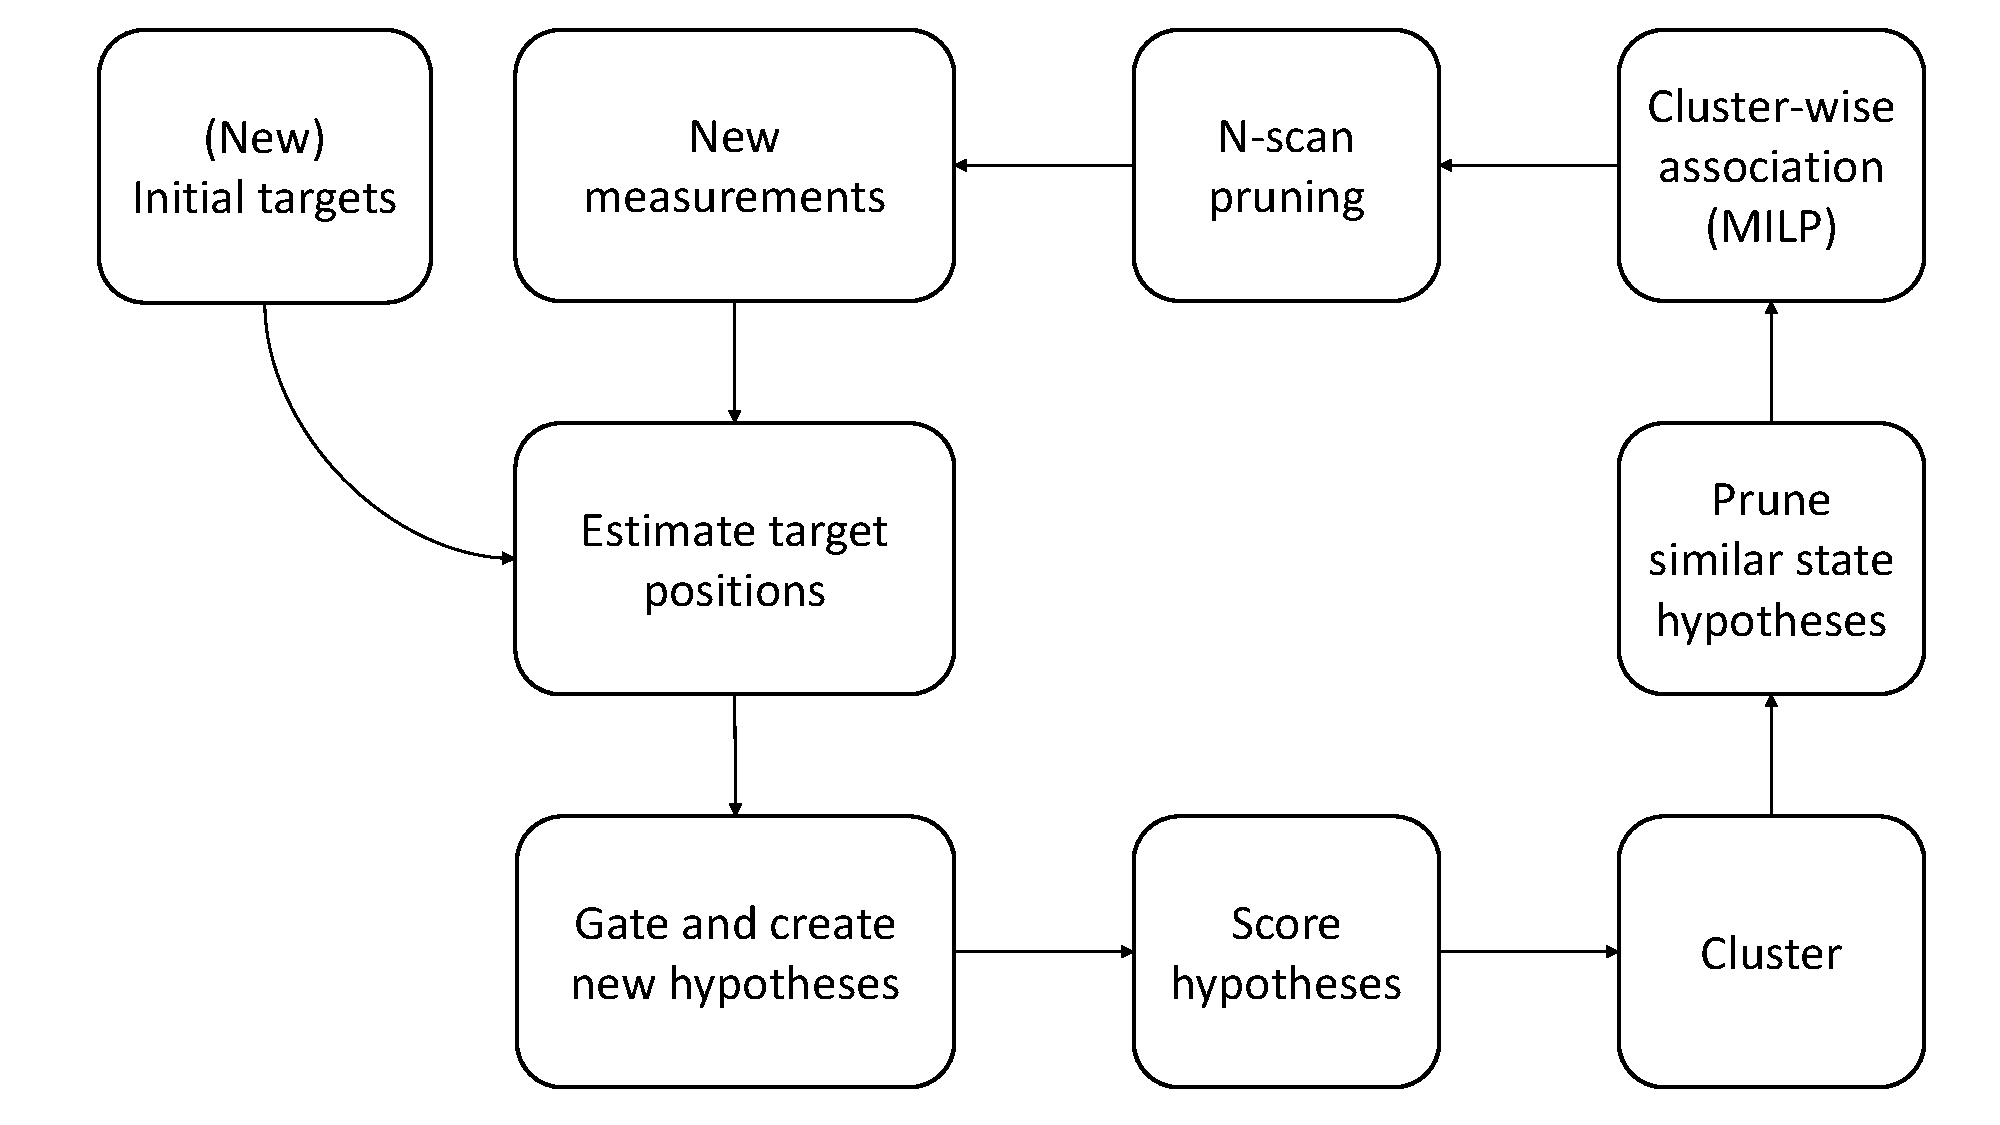
\includegraphics[width = .9\textwidth]{algorithm_flowchart.pdf}
\caption{Algorithm flowchart}
\label{fig:algorithm_flow}
\end{figure}

\subsection{State estimation}
When a new set of measurement is arriving, it is desirable to "guess" where the target might be before looking for matching measurements. This can be done though a model of the targets dynamics and a state estimator. For the purpose of tracking ships in a local frame (Cartesian plane), we compose a state vector with four states
\begin{equation}
\V{x} = \begin{bmatrix}
x & y & \dot{x} & \dot{y}
\end{bmatrix}^T
\label{eq:state_vector}
\end{equation}
where the change of velocity (acceleration) is assumed zero. The latest assumption is compensated with an increased system noise covariance in the model. For a linear system, a Kalman Filter is an optimal estimator which have the following time evolution assumptions.
\begin{equation}
\begin{split}
\V{x}(k+1) &= \M{\Phi} \V{x}(k) + \M{\Gamma} \V{w} \\
\V{z}(k) &= \M{H} \V{x}(k) + \V{v}
\end{split}
\label{eq:kalman_timeUpdate}
\end{equation}
where
\begin{equation}
\begin{split}
\M{\Phi} 	&= \text{the state transition matrix} \\
\M{\Gamma}	&= \text{the disturbance matrix} \\
\V{w}		&= \text{the process noise} \\
\M{H} 		&= \text{the measurement matrix} \\
\V{v} 		&= \text{the observation noise} \\
\end{split}
\end{equation}.
The procedure of estimating the target state at the next time step is according to the "time update" equations of the Kalman Filter.
\begin{equation}
\begin{split}
\V{\bar{x}}(k+1) 	&= \M{\Phi} \V{\hat{x}}(k) \\
\M{\bar{P}}(k+1)	&= \M{\Phi} \M{\hat{P}}(k)  \M{\Phi}^T + \M{Q} \\
\end{split}
\end{equation}
Where Q is the system covariance matrix. The model have the following parameters,
\begin{equation*}
\M{\Phi} =	\begin{bmatrix}
1 & 0 & T & 0 \\
0 & 1 & 0 & T \\
0 & 0 & 1 & 0 \\
0 & 0 & 0 & 1 \\
\end{bmatrix} \quad
\M{\Gamma} = \begin{bmatrix}
0 & 0 \\
0 & 0 \\
1 & 0 \\
0 & 1 \\
\end{bmatrix} \quad
\M{H} = \begin{bmatrix}
1 & 0 & 0 & 0 \\
0 & 1 & 0 & 0 \\
\end{bmatrix}
\end{equation*}
\begin{equation*}
\M{Q}	= \sigma_v^2 \begin{bmatrix}
\frac{T^3}{3} 	& 0 				& \frac{T^2}{2}	& 0 			\\
0 				& \frac{T^3}{3}  	& 0 			& \frac{T^2}{2}	\\
\frac{T^2}{2}	& 0					& T				& 0				\\
0				& \frac{T^2}{2}		& 0				& T				\\
\end{bmatrix} \quad
\M{R} = \sigma_r^2 \begin{bmatrix}
1 & 0 \\
0 & 1 \\
\end{bmatrix}
\end{equation*}
where $T$ is the time between the current and the previous measurement, $\sigma_v^2$ is the system velocity variance and $\sigma_r^2$ is the measurement variance. This model is very common due to its simplicity, and is used in among others \cite{Reid1978}, \cite{Coraluppi2000} and \cite{Brekke2012}.

\subsection{Gating}
To avoid calculating the likelihood for all possible combinations of targets and measurements, some sort of selection criteria is needed when creating new hypotheses. One way of doing this gating is to select all measurements that are within a certain confidence region (generally an ellipsoid), as done in \cite{Reid1978}.

\begin{gather*}
\M{B}	= \M{H} \M{\bar{P}} \M{H}^T + \M{R} \\
(\V{Z_m} - \M{H}\V{\bar{x}})^T	\M{B}^{-1} (\V{Z_m} - \M{H}\V{\bar{x}}) \leq \eta^2
\end{gather*}
Where $\eta$ is the gate size.  Chi-Square value with a given confidence interval and two degrees of freedom. For each measurement inside the region, calculate the a posteriori state and covariance using the "measurement update" equations in the Kalman Filter (\ref{eq:kalman_measurementUpdate}) and create a new hypothesis with this state and covariance as initial.

\begin{figure}[h]
\centering
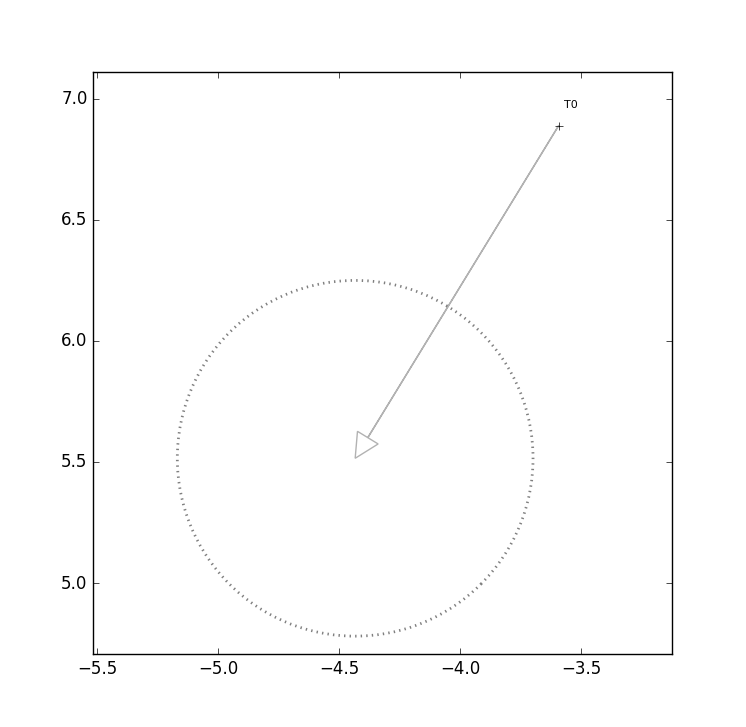
\includegraphics[width = .8\textwidth]{ex1-validationRegion}
\caption{Validation region}
\label{fig:validation_region}
\end{figure}

\begin{equation}
\begin{split}
\V{\tilde{y}}	&= \V{z} - \M{H} \V{\bar{x}} \\
\M{S}			&= \M{H} \M{\bar{P}} \M{H}^T + \M{R} \\
\M{K} 			&= \M{\bar{P}} \M{H}^T \M{S}^{-1} \\
\V{\hat{x}}(k) 	&= \V{\bar{x}} + \M{K} \V{\tilde{y}} \\
\M{\hat{P}}(k) 	&= \left( \M{I} - \M{K} \M{H} \right) \M{\bar{P}}
\end{split}
\label{eq:kalman_measurementUpdate}
\end{equation}

\subsection{Scoring}
Each hypothesis are scored according to \cite{Bar-Shalom2007}:
\begin{equation}
\begin{split}
NLLR_{t,j}(k) &= \frac{1}{2} \left[ \tilde{y}_k^T S_{tj}(k)^{-1} \tilde{y}_k \right] + \ln \frac{\lambda_{ex} |2 \pi S_{tj}(k)|^{1/2}}{P_{D_t}(k)} \\				
\tilde{y}_k &= z_j(k)-\hat{z}_t(k|k-1)
\end{split}
\end{equation}
where the cumulative NLLR is
\begin{equation}
l_t^k \triangleq \sum_{l=0}^k NLLR_{t,j(t,l)}(l)
\end{equation}

\subsection{Clustering}
Since the global problem of finding the optimal selection of hypotheses is growing exponentially with the number of hypotheses, it is computationally beneficial to split the problem into smaller problem. This can only be done to targets that does not share any measurements within the N-latest time step. This is done efficiently through breath-first-search or depth-first-search on a graph made from the hypothesis tree.

\subsection{Association}
When the targets are divided into independent clusters, each of them can be treated as a global problem where we want to minimize the cost of the selected hypothesis (leaf nodes), while fulfilling the constraints that each measurement can only me a part of one track and that we choose one and only one hypothesis for each target. Since it is undesirable (and physically impossible) to select fractions of a hypothesis, this becomes a linear integer optimization problem.

\subsection{N-scan pruning}
To keep the computational cost within reasonable limits, it is necessary to limit the amount of time steps backwards in time that the algorithm computes. This is done by removing all but the active hypothesis at the current root node, and assign the remaining hypothesis as new root node. 

\begin{figure}[ht]
\centering
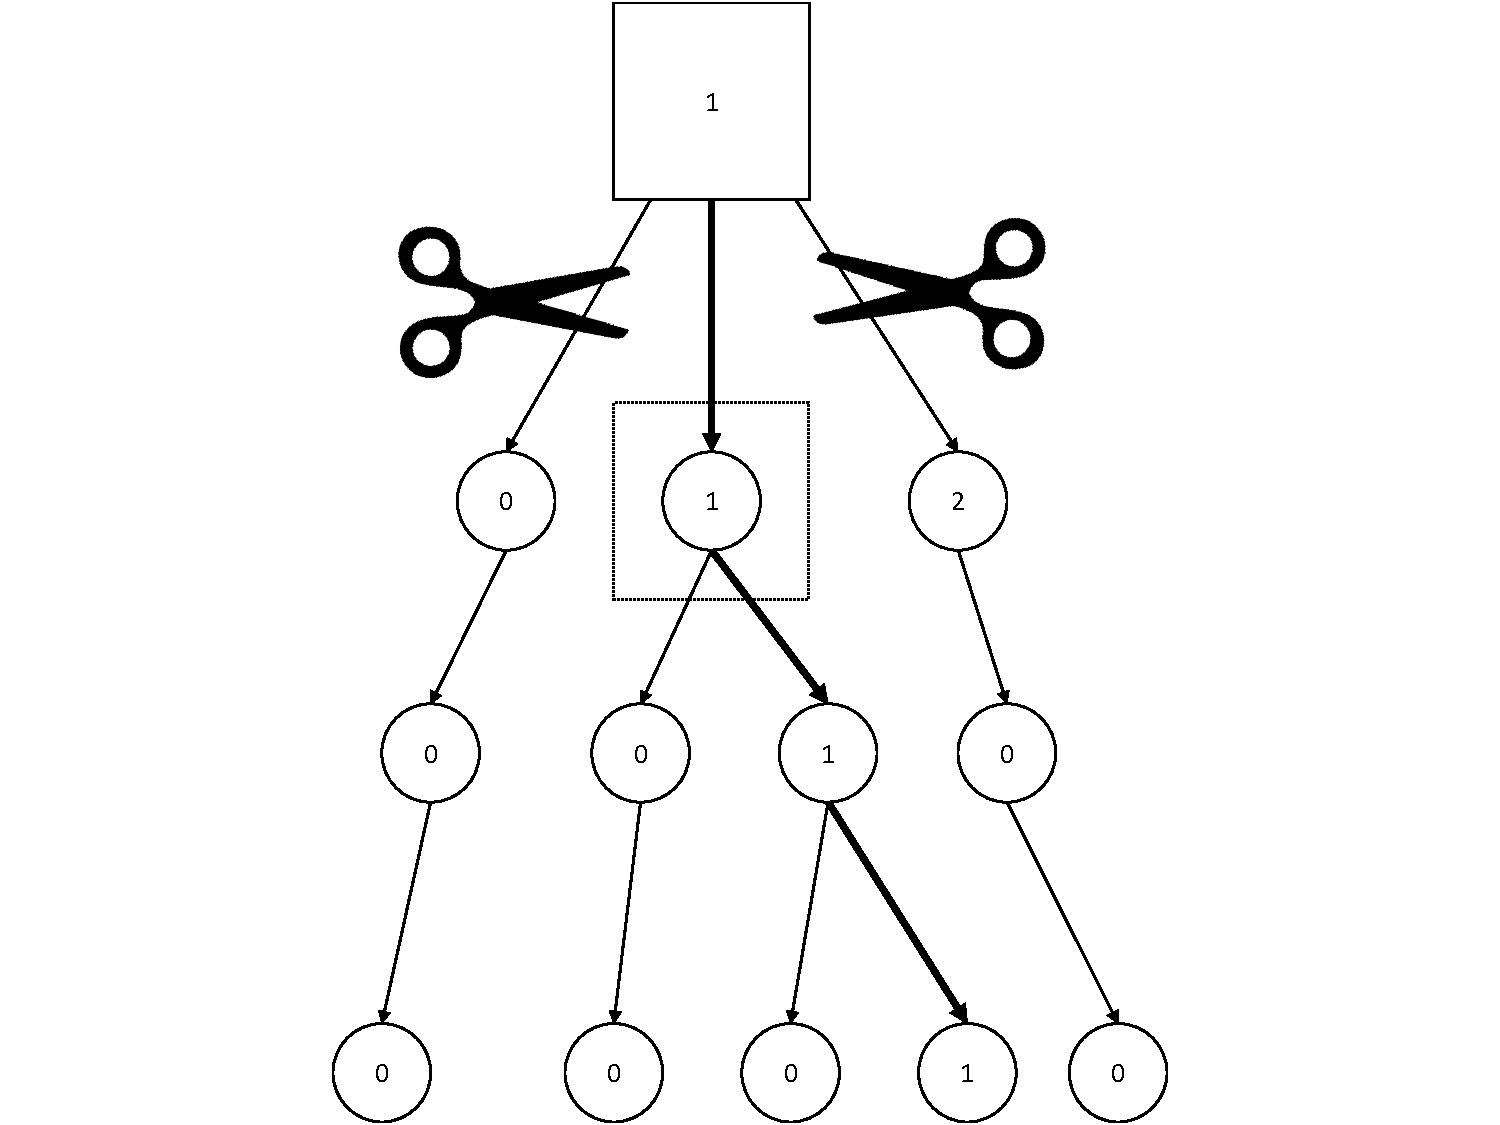
\includegraphics[width = .8\textwidth]{Pruned-tree.pdf}
\caption{Pruned track hypothesis tree}
\label{fig:pruned-hyp-tree}
\end{figure}